\documentclass[5p,times,authoryear]{elsarticle}
% ===========================================================================
% Shared preamble for every manuscript in this repository.
%
% Papers using it:
%   paper/            agriculture inventory
%   paper_nowcast/    agricultural nowcasting
%   paper_national/   the nine-sector national inventory
%   notes/<sector>/   one data note per non-agriculture sector
%
% It exists because paper/ and paper_nowcast/ began as copies of one another
% and had already drifted five lines apart before a third manuscript existed.
% Eleven copies would drift eleven ways, and a macro that renders differently
% in two papers is the kind of defect nobody notices until proof stage.
%
% \graphicspath is deliberately NOT set here - each manuscript sets its own
% after \input{...preamble}, because figures live beside the document.
% ===========================================================================

\usepackage[utf8]{inputenc}
\usepackage[T1]{fontenc}
\usepackage{amsmath,amssymb}
\usepackage{graphicx}
\usepackage{booktabs}
\usepackage{multirow}
\usepackage{siunitx}
\usepackage[colorlinks=true,citecolor=blue,linkcolor=blue,urlcolor=blue]{hyperref}
% Document-information metadata for every PDF in the bundle (the seventh review noted
% the shipped PDFs carried none). Documents that set their own \hypersetup{pdftitle=...}
% keep it - hyperref takes the LAST setting, and this shared block runs first. Full
% tagged-PDF (tagpdf / \DocumentMetadata) is deliberately not attempted here: the
% installed LaTeX toolchain's support is not uniform across sixteen documents, and a
% half-tagged bundle is worse than an honestly untagged one; deferred deliberately.
\hypersetup{
  pdfauthor={Rehan Ahmad, Pakistan Air Quality Initiative (PAQI)},
  pdfsubject={A reproducible ten-sector national greenhouse-gas inventory
              for Pakistan},
  pdfkeywords={Pakistan, greenhouse gas inventory, IPCC 2006 Guidelines, MRV,
               reproducible research, emissions, air pollutants},
}
\usepackage{caption}
\captionsetup[table]{position=below}
\usepackage{enumitem}
\usepackage{xcolor}
\usepackage{float}
\usepackage{placeins}
\usepackage{tabularx}
\usepackage{natbib}
\usepackage{tikz}
\usetikzlibrary{arrows.meta,positioning,fit,backgrounds}

\setlength{\emergencystretch}{3em}

% Looser float placement to prevent pile-up in two-column mode.
\renewcommand{\topfraction}{0.95}
\renewcommand{\bottomfraction}{0.85}
\renewcommand{\textfraction}{0.05}
\renewcommand{\floatpagefraction}{0.85}
\setcounter{topnumber}{4}
\setcounter{bottomnumber}{3}
\setcounter{totalnumber}{6}

% ---------------------------------------------------------------------------
% Custom shorthand: in macros.tex since the ESSD re-targeting, because the national
% article compiles under the Copernicus class and cannot take this preamble (the class
% loads its own packages) but needs exactly the same macros. This file inputs it so that
% every other manuscript keeps compiling unchanged.
%
% THREE relative paths, because \input resolves against the COMPILE DIRECTORY and not
% against this file, so the depth is a property of whoever is building:
%   ../paper_common      a manuscript compiled from one level down
%   ../../paper_common   papers/<sector>/ and notes/<sector>/
%   ../../../paper_common  paper_national/versions/<v>/, since the national paper was
%                          versioned - that move is what added this third arm, and the
%                          supplement failed with "../../paper_common/macros.tex not
%                          found" until it was here
% A fourth depth needs a fourth arm, which is the cost of keeping a bare `latexmk` in a
% manuscript directory working without a TEXINPUTS set for it.
% ---------------------------------------------------------------------------
\IfFileExists{../paper_common/macros.tex}%
  {\input{../paper_common/macros}}%
  {\IfFileExists{../../paper_common/macros.tex}%
    {% ===========================================================================
% paper_common/macros.tex - the shorthand every manuscript shares.
%
% Split from preamble.tex in the ESSD re-targeting: the national article now compiles
% under the Copernicus class, which loads its own packages and forbids most of what
% preamble.tex sets (geometry-like options, a second hyperref, placeins), but it needs
% exactly the same shorthand as the sector reports. The macros therefore live here, on
% their own, and preamble.tex inputs this file so that every other manuscript keeps
% compiling unchanged. A macro that renders differently in two documents is the defect
% this file exists to prevent; define it once.
%
% Requires: siunitx (for \DeclareSIUnit and \si) - the caller loads it.
% ===========================================================================

% Gas and pollutant names.
\newcommand{\COtwo}{CO\textsubscript{2}}
\newcommand{\COe}{CO\textsubscript{2}e}
\newcommand{\CHfour}{CH\textsubscript{4}}
\newcommand{\NtwoO}{N\textsubscript{2}O}
\newcommand{\NHthree}{NH\textsubscript{3}}
\newcommand{\NOx}{NO\textsubscript{x}}
\newcommand{\SOtwo}{SO\textsubscript{2}}
\newcommand{\PM}{PM\textsubscript{2.5}}
\newcommand{\MCF}{MCF}
\newcommand{\Mt}{\text{Mt~\COe}}
\newcommand{\tCha}{\si{\tonne\per\hectare}}
\newcommand{\AFOLU}{AFOLU}
\newcommand{\GLW}{GLW\,4}
\newcommand{\EFone}{EF\textsubscript{1}}

% siunitx: allow Mt, Tg, ha, head, yr, dB
\DeclareSIUnit{\head}{head}
\DeclareSIUnit{\yr}{yr}
\DeclareSIUnit{\dB}{dB}

% A file name is the one long unbreakable token these documents are full of -
% \texttt{waste\_air\_pollutants\_2024.csv} is wider than a two-column measure and TeX prints
% it past the margin rather than breaking it. Allowing a break AFTER each escaped underscore
% costs nothing and inserts no hyphen, which matters: a hyphenated file name is a wrong file
% name. This is one line because every such name in every document is written with \_.
\let\pkinvunderscore\_
\renewcommand{\_}{\pkinvunderscore\allowbreak}
}%
    {\input{../../../paper_common/macros}}}
% Long unbreakable strings - output filenames, module paths, URLs in \texttt - do not fit a
% two-column measure and TeX prints them past the margin rather than breaking them. Nothing
% read the log, so 47 of those overruns shipped across seven documents. Emergency stretch lets
% the paragraph loosen instead, and \texttt is taught to break at the punctuation these names
% actually contain.
\emergencystretch=6em


\graphicspath{{figures/}}
\begin{document}
\begin{frontmatter}
\title{Supplementary Methods: From Fuel Customers to Flight Geography}
\author[paqi]{Rehan Ahmad}
\address[paqi]{Pakistan Air Quality Initiative (PAQI), Karachi, Pakistan}
\end{frontmatter}
%% Generated by scripts/make_release_cover.py; says which release this supplement documents.
%% GENERATED by scripts/make_release_cover.py from outputs/release_manifest.json.
%% Do not edit: the edit will be overwritten and CI diffs the result.
\newcommand{\ReleaseCover}{%
\begin{center}\small
\setlength{\fboxsep}{4pt}%
\fbox{\begin{minipage}{\dimexpr\linewidth-2\fboxsep-2\fboxrule\relax}\footnotesize
\textbf{Release provenance.} This document describes PakEmis under the period, configuration and source boundaries specified in its methods. The identifiers below link it to the accompanying products and source register.\\[2pt]
\begin{tabular}{@{}p{0.32\linewidth}@{\hspace{0.03\linewidth}}p{0.65\linewidth}@{}}
Release version & \texttt{1.0.0rc69} \\
Commit & \texttt{d8d874622f9a} \\
Reporting period & July 2015--June 2025 (ten fiscal years) (2015-07-01 to 2025-06-30) \\
Reference & S\_TAN (household survey; TAN nitrogen) \\
FY2023--24 total & 444.61 Mt \COe{} (AR5) under S\_TAN, the reference; 449.85 Mt under L\_TAN \\
Release manifest & \texttt{ac0ffe93ad9fcd88} (SHA-256 of \texttt{outputs/release\_manifest.json}, first 16) \\
Source manifest & \texttt{c1be6d314cfce1ea} (SHA-256 of \texttt{data/manifests/source\_manifest.csv}, first 16) \\
Data-description article & \texttt{paper\_national/} (ESSD, in preparation), same release
\end{tabular}
\end{minipage}}
\end{center}}

\ReleaseCover


\section{Source-neutral flight-stage contract}

All provider-specific adapters terminate at one validated record. Required fields are a stable
flight identifier, fiscal year, origin and destination ICAO codes, domestic/international
boundary, activity count, record granularity, source tier, operator, aircraft type, trajectory
quality, imputation method and source reference. Optional fields include date and timestamps,
callsign, ICAO24, registration, engine, passengers, cargo, great-circle and trajectory distance,
and taxi, take-off, climb, cruise, descent and landing fuel. Phase fuel must sum to total fuel;
the geography implied by endpoints must agree with the stored boundary.

Four tiers are enforced. Tier A is an observed flight and trajectory; Tier B is an observed
flight stage with a synthetic trajectory; Tier C is a reconstructed annual route stratum; Tier
D is aggregate residual activity. Tiers A and B require flight-stage granularity and timestamps;
Tier C cannot contain invented dates; Tier D cannot be assigned fictional endpoints. ADSB.lol,
OpenSky \citep{adsblolhistory,schaefer2014opensky}, a future PCAA operational export and a
canonical CSV/Parquet import therefore feed the same emissions and accounting code.

\section{Provisional route and aircraft reconstruction}

The FY2023--24 route graph contains only routes with contemporaneous timetable, airline-report
or route-announcement evidence. Each evidence record carries applicable dates, operator, source
class and URL. An iterative constrained allocation balances airport origin and destination
margins. A joint linear allocation then assigns operator departures without exceeding either an
airline control or route capacity. Airport, route and operator deficits are retained as Tier D.

Let $x_{aij}$ denote annual stages by operator $a$ from airport $i$ to $j$. The central matrix
minimises deviation from documented seed weights subject to airport outflow and inflow margins,
operator departure controls, reciprocal-route support and non-negativity. Over the same
feasible set, separate programmes minimise and maximise $\sum_{aij}x_{aij}d_{ij}$, where
$d_{ij}$ is great-circle distance. The resulting matrices isolate route-graph uncertainty
without changing activity totals or inventing unsupported links.

Aircraft are assigned as probabilities by airline and route, not as invented registrations.
OpenAP \citep{sun2020openap} provides synthetic phase profiles for supported types. Unsupported
types remain visibly unfuelled in the native model and receive a separate ICAO calculator
imputation only in the coverage-completion experiment \citep{icaoicec2024}. Low, central and
high payload configurations change dispatch mass through passengers, cargo and mail. Detour,
taxi time and weather are varied separately in the Monte Carlo so their effects are identifiable;
the main paper reports the central common-support comparison.

The installed OpenAP deterministic generator documents cruise range in kilometres but compares
the supplied value with an internally metre-scaled trajectory. The adapter therefore identifies
the installed convention with a bounded probe, selects the highest feasible cruise altitude on
short routes and requires generated horizontal distance to match the detoured route within 3\%
or 5 km. It also requires profile duration to increase materially with route length and each
phase-fuel sum to equal total fuel. These invariants detected the earlier near-route-invariant
profiles and remain executable regression checks.

\section{PCAA payload and departure controls}

Central payload is no longer defined by one generic MTOW fraction. For each operator and
boundary, PCAA embarked passengers are divided by published departures; assigned aircraft-
family shares supply weighted seats; loaded cargo and mail are divided by the same departure
control. Table~\ref{tab:payload-controls} reports the domestic values used by M2. Low and high
cases use 62.5\% and 87.5\% passenger loads unless the observed centre lies beyond those
screening values; this guarantees low $\leq$ central $\leq$ high up to physical seat capacity.
The outputs retain a warning rather than silently treating an impossible load as valid.

\begin{table}[htbp]
\centering
\scriptsize
\begin{tabular}{@{}lrrrr@{}}
\toprule
\textbf{Operator} & \textbf{Pax/dep.} & \textbf{Seats} & \textbf{Implied load} & \textbf{Cargo+mail kg/dep.} \\
\midrule
Airblue (ABQ) & 170.4 & 194 & 0.878 & 0 \\
Fly Jinnah (FJL) & 156.8 & 180 & 0.871 & 811 \\
PIA & 109.5 & 147 & 0.745 & 723 \\
SereneAir (SEP) & 173.1 & 189 & 0.916 & 2187 \\
AirSial (SIF) & 174.4 & 180 & 0.969 & 1308 \\
\bottomrule
\end{tabular}
\caption{Domestic operator-average payload controls. They constrain, but do not claim to
observe, route-specific payload.}
\label{tab:payload-controls}
\end{table}

The airline report contains 19,752 domestic departures and arrivals, versus 20,300 stages from
airport movements divided by two (difference $-548$, or $-2.7$\%). Internationally, 45,723
published departures compare with 47,633.5 half-movements (difference $-1,910.5$, or $-4.0$\%);
departures exceed arrivals by 526. The incomplete international reconstruction assigns only
2,510 of PIA's 9,009 departures and therefore produces an above-capacity warning if its partial
aircraft mix is applied to all reported passengers. That warning is retained as a coverage
diagnostic and is not used to alter the domestic payload model.

\section{Extended reconciliation diagnostics}

Figure~\ref{fig:supp-source-bridge} retains the full graphical source-row bridge. The main
paper reports the same values in a compact conservation table so that the empirical argument
is not interrupted by every structural destination.

\begin{figure*}[htbp]
\centering
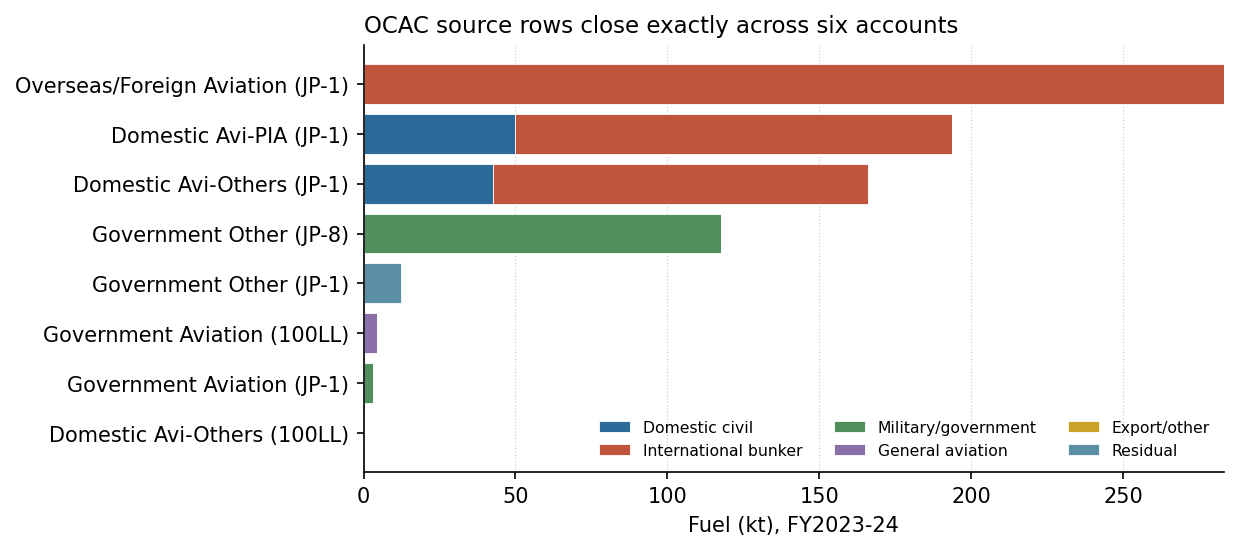
\includegraphics[width=0.92\textwidth]{aviation_source_bridge.png}
\caption{FY2023--24 OCAC rows assigned across six non-overlapping accounts under the
OECD-calibrated resident share.}
\label{fig:supp-source-bridge}
\end{figure*}

The monthly and extended annual comparisons in Figure~\ref{fig:supp-temporal} show why the
latest annual ratios are treated as evidence rather than a permanent identity. Monthly
combined ratios fluctuate around unity; over the full complete OECD overlap, combined closure
improves while resident and foreign discrepancies retain opposite signs.

\begin{figure*}[htbp]
\centering
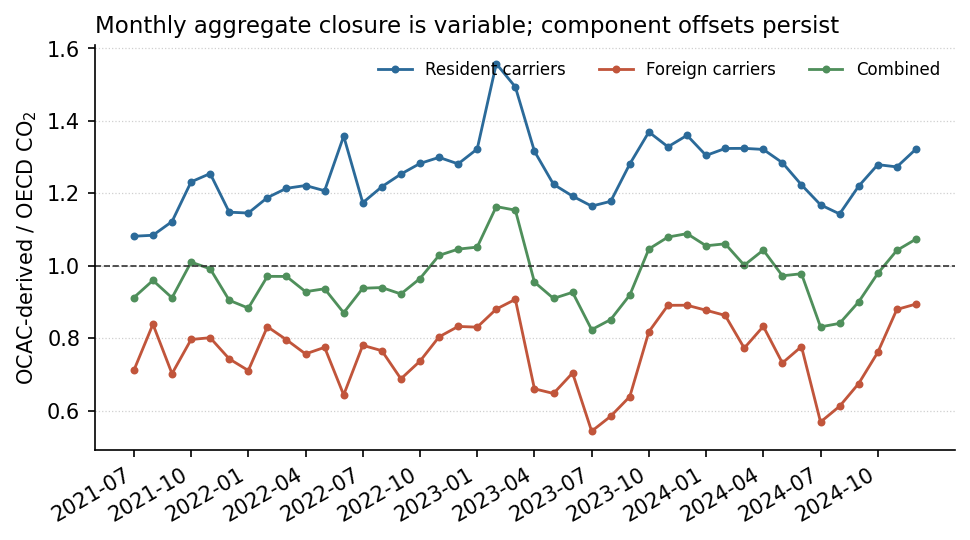
\includegraphics[width=0.47\textwidth]{aviation_monthly_closure.png}\hfill
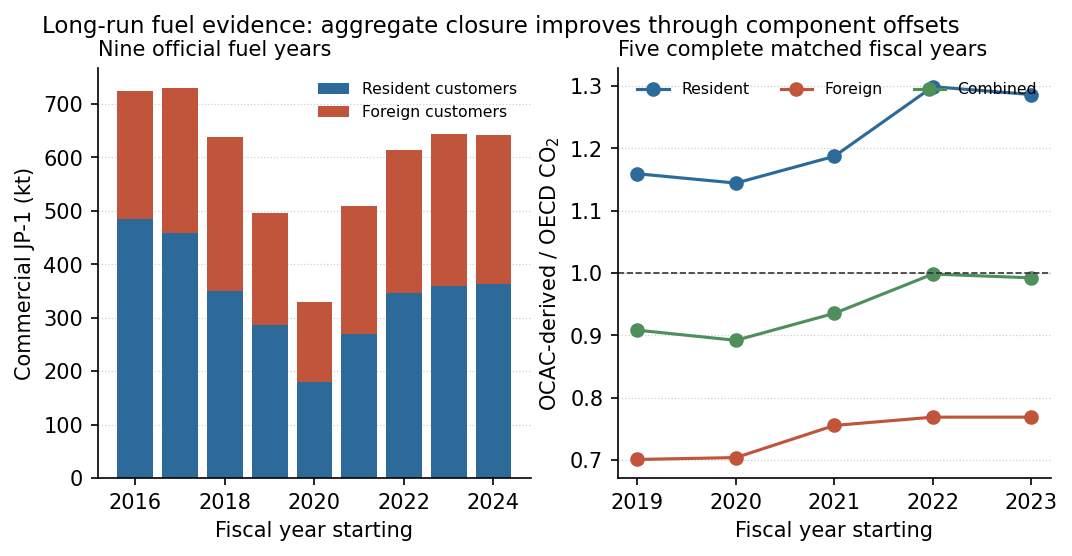
\includegraphics[width=0.50\textwidth]{aviation_long_run_controls.png}
\caption{Supporting temporal evidence. (a) Monthly OCAC-derived to OECD \COtwo{} ratios.
(b) Nine annual fuel accounts and five complete fiscal-year component comparisons.}
\label{fig:supp-temporal}
\end{figure*}

\section{Comparison independence and model diagnostics}

Table~\ref{tab:supp-independence} gives the full comparison registry underlying the compact
source-role table in the main paper. Calibration, external provenance and statistical
independence are separate attributes.

\begin{table*}[htbp]
\centering
\scriptsize
\begin{tabular}{@{}p{0.22\textwidth}p{0.19\textwidth}p{0.25\textwidth}p{0.13\textwidth}p{0.10\textwidth}@{}}
\toprule
\textbf{Comparison} & \textbf{Purpose} & \textbf{Shared input} & \textbf{Independence} & \textbf{Calibration} \\
\midrule
Movement vs OECD domestic & External territory comparison & Possible ICAO performance conventions & Partial & No \\
Fuel bridge vs OECD domestic & Partition consistency & OECD resident share used directly & None & Yes \\
OCAC total vs OECD combined & Gross-boundary closure & Carbon conversion only & Large & No \\
Pakistan CRT vs OECD & Official-boundary diagnostic & Inventory year only & Large & No \\
PCAA airports vs Climate TRACE & Spatial corroboration & Possible surveillance/performance inputs & Partial & No \\
ADSB.lol vs PCAA daily rate & Coverage pilot & Airport coordinates only & Large but incomplete & No \\
ERA5 vs OpenAP still air & Weather sensitivity & Same synthetic route/fuel & Not validation & No \\
PCAA movements vs passengers & Movement-divisor check & PCAA reporting system & Targeted & No \\
\bottomrule
\end{tabular}
\caption{Complete independence and shared-input registry.}
\label{tab:supp-independence}
\end{table*}

\begin{figure*}[htbp]
\centering
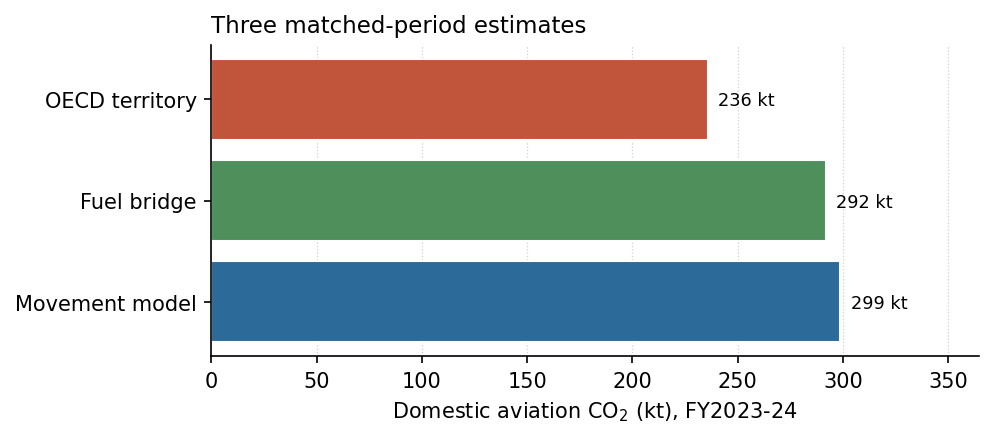
\includegraphics[width=0.31\textwidth]{aviation_reconciliation.png}\hfill
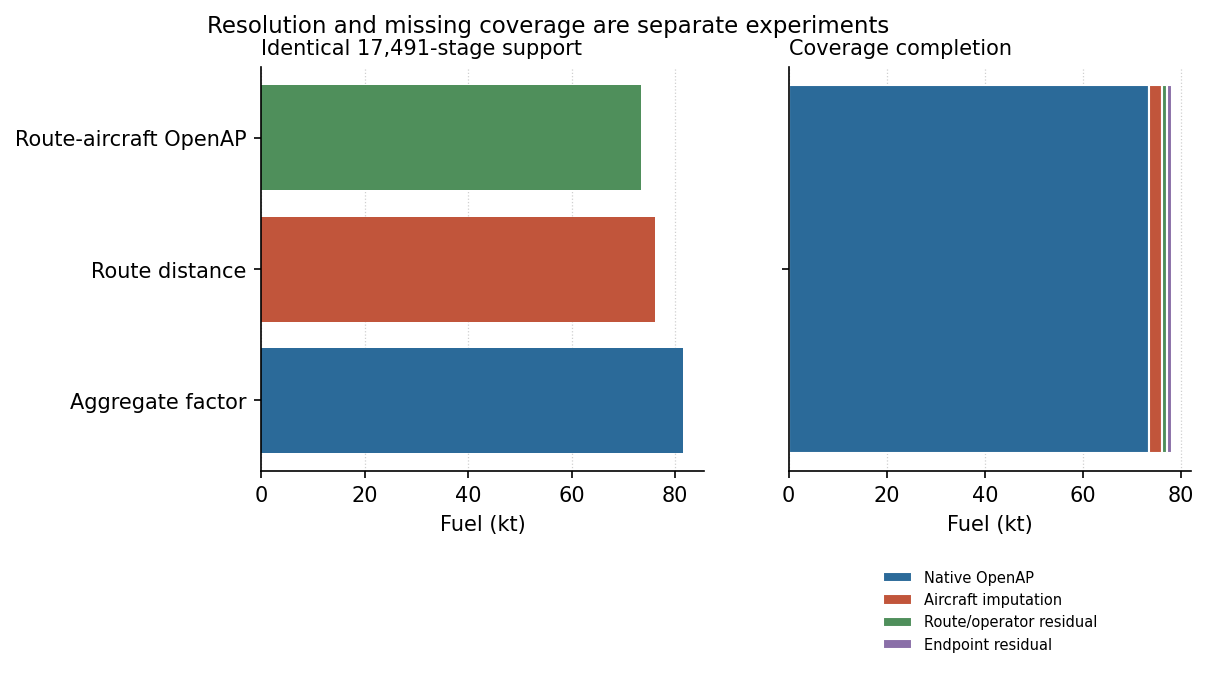
\includegraphics[width=0.31\textwidth]{aviation_resolution_ladders.png}\hfill
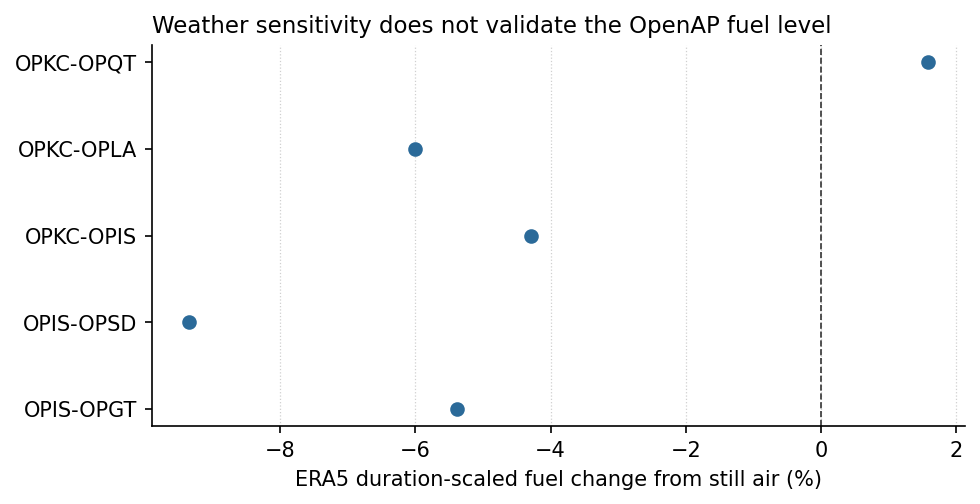
\includegraphics[width=0.31\textwidth]{aviation_era5_weather_audit.png}
\caption{Implementation diagnostics moved from the main narrative. (a) Calibrated bridge,
aggregate movement and OECD domestic comparison. (b) Common-support and coverage-completion
ladders. (c) ERA5 duration sensitivity for representative routes.}
\label{fig:supp-model-diagnostics}
\end{figure*}

\section{Observed-data adapters and activation gate}

The implemented OpenSky adapter queries flight records first and state vectors only for selected
flight identifiers and time bounds. The ADSB.lol adapter instead streams ODbL daily readsb
archives, honours the trace new-leg bit, links only low-altitude airport candidates and emits
the same Tier-A records without redistributing the underlying trace database
\citep{readsbjson}. Coverage is evaluated against PCAA airport and airline controls by month,
boundary and operator. An observed ledger may replace the calibrated OECD
resident share only when domestic and international route and fuel coverage each exceed 90\%
for both OCAC resident customer groups. Below that gate, modelled fuel is a partial diagnostic
and uncovered OCAC fuel remains residual. This rule prevents a high-coverage domestic sample
and low-coverage international sample from producing a biased customer split.

\section{ADSB.lol coverage-pilot result}

The selected dates are 15 August 2023, 15 November 2023, 15 February 2024 and 15 May
2024. Their release assets total 7.05 GiB. Streaming 219,596 trace members yields 1,543
aircraft traces and 4,281 legs in the broad regional candidate rectangle, but zero low-altitude
links to a Pakistani airport and therefore zero canonical Tier-A stages. One malformed member
per archive is counted as a parse failure. The nearest horizontal candidate is 0.25 km from a
catalogued airport; it is rejected by the altitude-relative gate. Only these aggregate counts,
release identifiers, file sizes, licence and method are distributed. The raw trace cache and a
derived reusable flight database are withheld pending ODbL derivative-database review.

Two positive controls use the same canonical-stage code. A synthetic OPKC--OPLA trace emits one
Tier-A domestic stage with the expected endpoints. The unmodified 15 August archive, scanned
with the identical 35-km and elevation-relative gate around OMDB, emits 700 airport-linked legs;
686 have callsigns and 697 have aircraft types. Both controls pass. The zero Pakistan result is
therefore evidence about this sample's coverage, not a silent parser or endpoint-gate failure.

\section{Official-reporting extraction}

The official CRT ZIP is read in memory and the energy workbook is selected by exact filename.
The extractor takes emissions from Table 1, domestic activity from Table 1.A(a)s3 and bunker
activity plus the domestic/international distribution from Table 1.D. It asserts that both
aviation categories, both activity cells and the distribution exist. The output retains the
ZIP SHA-256, reported fuel label and jet-kerosene notation. BTR/NC3 narrative entries are a
separate normalized control because their rounded printed values cannot be treated as CRT-
precision observations.

The archived file is \texttt{PAK\_CRT\_2024.zip}. Its SHA-256 is printed as two consecutive
32-character blocks:
\begin{center}\small\ttfamily
afba70d10be0694aea6b2ba2cec311e1\\
49473346daa206319138185c190e8f38
\end{center}
The selected workbook is \texttt{ENERGY-PAK-CRT.xlsx}; its two consecutive SHA-256 blocks are:
\begin{center}\small\ttfamily
ca504f7eb0894573d790b1b4c08576d4\\
fbe795acd56ef5e5c4120b0d3897a944
\end{center}
Table~\ref{tab:crt-extract} reproduces the cells carrying the central interpretation. The
generated cell-audit CSV contains all 21 pinned cells, including CH4, N2O and \COe{}, along with
raw data type, formula, unit, transformation, transformed value and notation key.

\begin{table*}[htbp]
\centering
\scriptsize
\begin{tabular}{@{}lllll@{}}
\toprule
\textbf{Cell} & \textbf{Field} & \textbf{Raw value} & \textbf{Unit} & \textbf{Transformation} \\
\midrule
Table1!C25 & Domestic \COtwo{} & 654.065328 & kt \COtwo{} & $\times1000$ to t \\
Table1!C53 & International \COtwo{} & 163.516332 & kt \COtwo{} & $\times1000$ to t \\
Table1.A(a)s3!C17 & Domestic aviation gasoline & 9343.7904 & TJ & Retain \\
Table1.A(a)s3!H17 & Domestic gasoline \COtwo{} & 654.065328 & kt \COtwo{} & $\times1000$ to t \\
Table1.A(a)s3!C18/H18 & Domestic jet kerosene & NE / NE & Notation key & Retain NE \\
Table1.D!C12 & International aviation gasoline & 2335.9476 & TJ & Retain \\
Table1.D!G12 & International gasoline \COtwo{} & 163.516332 & kt \COtwo{} & $\times1000$ to t \\
Table1.D!C11/G11 & International jet kerosene & NE / NE & Notation key & Retain NE \\
Table1.D!L9 & Domestic distribution & 80.00000000000001 & percent & Retain exact \\
Table1.D!M9 & International distribution & 19.999999999999986 & percent & Retain exact \\
\bottomrule
\end{tabular}
\caption{Reproduced extract from the official CRT workbook. No value was manually transcribed
into the normalized inventory: the extractor reads and asserts these cells.}
\label{tab:crt-extract}
\end{table*}

\section{ERA5 weather-duration audit}

The reproducible CDS request selects temperature and horizontal winds at 250, 500 and 850 hPa
over 23--38$^\circ$N, 60--79$^\circ$E at 12 UTC on the 15th of each FY2023--24
month. Bilinear interpolation samples 21 equally spaced points on six representative routes.
At 250 hPa, wind projected on route bearing adjusts airborne duration; taxi fuel is unchanged
and remaining OpenAP fuel scales with duration. Across 18 central route--aircraft strata the
mean change is $-3.90$\% (range $-9.35$\% to $+1.59$\%), comparable to the corrected 3.5\%
common-support M1--M2 difference. It does not model dispatch mass, reserves or wind-optimal
routing and does not rerun the OpenAP equations with meteorological state.

\section{Airport Air-Pollutant Layer}
\label{sec:air}

NOx, CO and HC are recalculated from representative aircraft--engine combinations in the ICAO
Engine Emissions Databank \citep{icaoeedb}. The mapping is complete for the commercial fleet,
but every row is marked imputed because aircraft registrations and actual engine fits are not
available. The turboprop fallback and fuel-based SO2, PM2.5 and black-carbon factors are
reported separately \citep{emep2023aviation}.

These remain LTO mass estimates rather than a complete airport micro-inventory. Standard fleet
shares stand in for airport-specific aircraft assignments, and actual taxi time, APU, ground
support, brake and tyre sources are not estimated. Consequently the layer supports screening
and method development, not claims about population exposure. A defensible airport inventory
will require registration-to-engine matching and observed times in mode as recommended by ICAO
Doc~9889 \citep{icao9889}.

\begin{figure}[htbp]
\centering
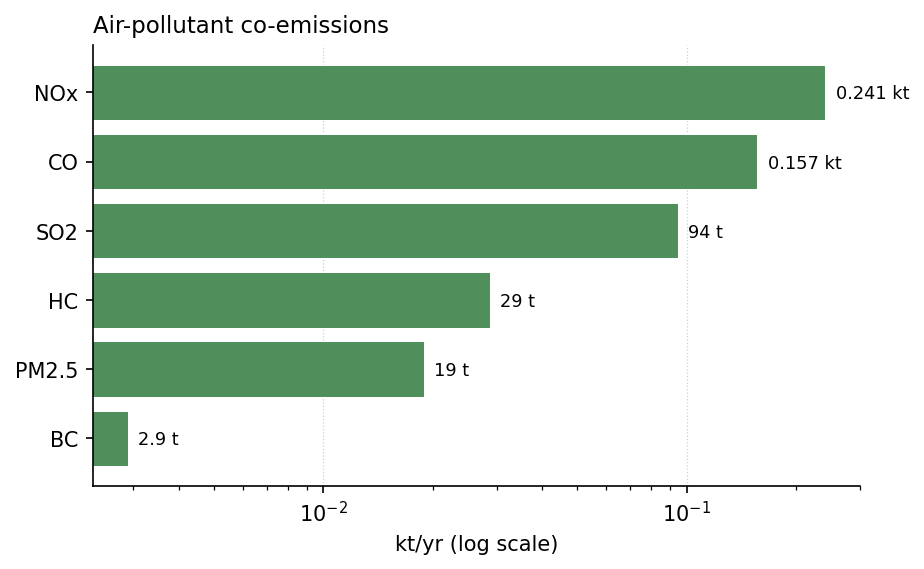
\includegraphics[width=\linewidth]{aviation_air.png}
\caption{Domestic main-engine LTO pollutants on a logarithmic mass axis. Values use
representative, explicitly imputed aircraft--engine mappings.}
\label{fig:air}
\end{figure}


\section{Products intentionally withheld without observed trajectories}

No route-altitude grid, physical emissions-over-Pakistan product, observed taxi-time inventory,
registration-to-engine inventory or airport micro-inventory is generated from Tier C records.
Once Tier A/B records are available, the existing product layer can emit airport LTO, climb,
cruise and descent segments, altitude bins and monthly gridded fields. National UNFCCC domestic,
international bunker, resident-carrier and physical-airspace accounts remain separate products.

\section{Fallback coverage}

The documented graph allocates 20,097.5 of 20,300 domestic stages. Named domestic-airline
assignment covers 19,752 departures. Native OpenAP fuel profiles cover 17,491.2 stages. The
resident-carrier international reconstruction covers 4,653 of 16,701 departures (27.9\%), so it
does not pass the activation gate. These are coverage diagnostics, not claims that reconstructed
records are observed flights.

\section{Reproduction}
\label{app:repro}

\begin{verbatim}
pip install -e '.[aviation,gis]'
make aviation-study
make figures sync-figures
make test
\end{verbatim}

The study target rebuilds official controls, the provisional fallback and every reconciliation
product, and writes the tables below. Each is named: the paragraph this replaces described them
by size---"\num{42} monthly comparison rows", "\num{240} monthly source rows"---which told a
reader how large each output is without saying which file it is.

\begin{itemize}\itemsep2pt
\item \texttt{aviation\_ocac\_monthly.csv}: \num{240} monthly source rows: reported tonnes by customer category and fuel type, each with its source URL, local file, SHA-256 hash and revision note.
\item \texttt{aviation\_ocac\_cumulative\_monthly.csv}: the same source on a cumulative basis.
\item \texttt{aviation\_ocac\_annual\_summary.csv}: \num{9} annual OCAC summaries: resident commercial, foreign commercial and government JP-1 by fiscal year.
\item \texttt{aviation\_monthly\_reconciliation.csv}: \num{42} monthly comparison rows, OCAC against OECD \COtwo{} with the resident and foreign ratios.
\item \texttt{aviation\_ocac\_oecd\_annual\_comparison.csv}: the annual OCAC--OECD comparison, of which \num{5} years are complete: the others match six months each and are marked partial rather than dropped.
\item \texttt{aviation\_annual\_component\_comparison.csv}: the same comparison by component, with the role each component plays in it and the government JP-1 that is excluded.
\item \texttt{aviation\_\allowbreak bridge\_\allowbreak source\_\allowbreak rows\_\allowbreak all\_\allowbreak scenarios.csv}: every source row under every scenario, with its IPCC domestic, international-bunker, military 1A5b and general-aviation assignment.
\item \texttt{aviation\_fuel\_bridge\_fy2023\_24.csv}: the reference year's fuel bridge on the same assignments.
\item \texttt{aviation\_reconciliation\_fy2023\_24.csv}: the reference-year reconciliation: domestic, international and residual fuel against the bottom-up domestic estimate.
\item \texttt{aviation\_model\_resolution\_fy2023\_24.csv}: how much of the domestic flight population each model resolves---stages modelled against stages total, with the resulting coverage share.
\item \texttt{aviation\_common\_support\_ladder.csv}: the common-support ladder, each step's stage and fuel coverage under one activity definition.
\item \texttt{aviation\_two\_year\_replication.csv}: the two-year replication, including the route coverage share and the network assumption behind it.
\item \texttt{aviation\_timeseries\_2006\_fy2023\_24.csv}: domestic LTO cycles and \COe{} by fiscal year from 2006.
\item \texttt{aviation\_uncertainty\_inputs\_complete.csv}: the complete input register: central value, 95\,\% range, distribution, applicable model, correlation group and uncertainty class per variable.
\item \texttt{aviation\_m2\_uncertainty\_intervals.csv}: the intervals by model, route graph and completion method, with the draw count and seed.
\item \texttt{aviation\_\allowbreak m2\_\allowbreak uncertainty\_\allowbreak contributions.csv}: what each uncertainty group contributes, as the variance reduction from freezing it.
\item \texttt{aviation\_uncertainty\_sensitivity.csv}: the one-at-a-time sensitivity: each variable's low and high case and its maximum absolute effect.
\end{itemize}

The run also writes the official UNFCCC extraction, the Climate TRACE fiscal and airport
products, the route bounds, the completion ladder, the weather and observed-coverage pilots,
the independence matrix, the QA table and a hash manifest.

The sector's own registered result is written by \texttt{make aviation} rather than by the
study target, and its five tables were named in neither list above---not described and left
nameless, simply absent, which is the harder omission to notice:

\begin{itemize}\itemsep2pt
\item \texttt{aviation\_\allowbreak by\_\allowbreak stream\_\allowbreak fy2023\_\allowbreak 24.csv}: the registered stream ledger---category,
  subitem and gas with the fossil flag, gigagrams, both common-GWP vintages and the
  uncertainty per row.
\item \texttt{aviation\_\allowbreak fuel\_\allowbreak constrained\_\allowbreak by\_\allowbreak stream\_\allowbreak fy2023\_\allowbreak 24.csv}: the same ledger
  under the fuel constraint, which is the comparison the bridge exists to make.
\item \texttt{aviation\_provincial\_fy2023\_24.csv}: the province-level AR5 total.
\item \texttt{aviation\_monthly\_fy2023\_24.csv}: the twelve-month layer, each month's share
  with the emissions it implies in both vintages and the temporal method and basis behind the
  shape.
\item \texttt{aviation\_completeness\_fy2023\_24.csv}: one row per source stream with its
  status and the note that qualifies it.
\end{itemize}

\section{Accounting and QA/QC guarantees}

Automated tests require: OCAC JP-1 totals of \SI{633879}{\tonne} and
\SI{658334}{\tonne} in the two fiscal years; exact closure of every source row; non-negative,
non-overlapping assignments; monthly sums equal to their reported cumulative controls and any
final-report revision remains explicit; calendar/fiscal
benchmark periods; reproducible Monte Carlo draws; separate structural scenarios; route-bound
ordering; identical common support; coverage completion to 20,300 stages; international memo
exclusion; distinct LTO and full-flight bunker quantities; representative-engine provenance and
imputation flags; and agreement between generated outputs and manuscript values.

\begin{table*}[htbp]
\centering
\scriptsize
\begin{tabular}{@{}p{0.23\textwidth}p{0.13\textwidth}p{0.17\textwidth}p{0.23\textwidth}p{0.09\textwidth}@{}}
\toprule
\textbf{Variable} & \textbf{Central} & \textbf{Range/distribution} & \textbf{Source or correlation group} & \textbf{Class} \\
\midrule
Official domestic movements & 40,600 & Reported; not sampled & PCAA FY2023--24 & Parametric control \\
M0 aggregate activity/fleet representation & 1.0 & $\pm60$\%; lognormal & Legacy M0 only & Parametric \\
Constrained route mean & 486.5 nmi & 485.2--503.0; bounded & PCAA margins/supported graph & Structural \\
M0 representative stage & 550 nmi & $\pm35$\%; lognormal & ICAO route sample; all stages & Parametric \\
Airline--aircraft shares & Route shares & Categorical draw & Fleet histories; operator--unordered route & Parametric within M2 \\
OpenAP payload & PCAA passengers, cargo, mail & Observed-centred bounded triangular & Operator and aircraft family & Parametric \\
Route detour & 1.08 & $\pm10$\%; lognormal & Shared reciprocal route & Parametric \\
Taxi-in/out & 420/900 s & $\pm50$\%; lognormal & Shared airport & Parametric \\
Unsupported-aircraft fuel & ICAO factor & OpenAP/ICAO; discrete & Aircraft family & Structural \\
Fuel carbon conversion & 3.16 t/t & $\pm5$\%; lognormal & IPCC/ICAO; all fuel & Parametric \\
CH4 factor & 0.5 kg/TJ & $\pm80$\%; lognormal & IPCC; all fuel & Parametric \\
N2O factor & 2.0 kg/TJ & $\pm110$\%; lognormal & IPCC; all fuel & Parametric \\
Customer to geography & OECD-calibrated & Literal/movement/carrier cases & OCAC/PCAA/OECD source row & Structural \\
International stage coverage & 27.9\% & Partial vs residual; discrete & Operator--route & Structural \\
Weather duration adjustment & Still air & ERA5 audit; empirical resampling & Global secondary interval & Parametric sensitivity \\
\bottomrule
\end{tabular}
\caption{Complete uncertainty-input register. The generated CSV additionally records the
applicable model and exact source string. Reported controls are conditional on source quality;
structural choices are not pooled into a confidence interval.}
\label{tab:uncertainty-register}
\end{table*}

\begin{table*}[htbp]
\centering
\scriptsize
\begin{tabular}{@{}p{0.36\linewidth}p{0.16\linewidth}p{0.27\linewidth}@{}}
\toprule
\textbf{Stream/product} & \textbf{Status} & \textbf{Boundary note} \\
\midrule
Scheduled domestic full flight & Estimated & M0/M1/bridge; M2 diagnostic \\
International bunkers & Estimated & Full-flight bridge memo \\
International airport LTO & Estimated & Separate local-air product \\
General aviation/training & Partial & 100LL priced as a memo row; activity unresolved \\
Military/government & Memo & JP-8/government candidates, priced as memo rows \\
Helicopters & Not estimated & No classified activity \\
APU/ground support & Not estimated & Airport survey required \\
Main-engine LTO pollutants & Estimated & Representative engines \\
Cruise pollutants/non-\COtwo{} effects & Not estimated & Separate research product \\
Tyre and brake wear & Not estimated & No local activity assignment \\
\bottomrule
\end{tabular}
\caption{Completeness matrix. Known omissions remain explicit rather than being absorbed into
``non-commercial aviation''.}
\label{tab:completeness}
\end{table*}

The source hierarchy is IPCC Volume~2 Chapter~3 for greenhouse-gas boundaries and factors
\citep{ipcc2006energy}; OCAC for petroleum sales \citep{ocacaviation}; PCAA for movements and
passengers \citep{pcaaairports2024,pcaaairlines2024}; Pakistan's BTR, NC3 and CRT for official
national reporting \citep{pakbtr2024,paknc32025,pakcrt2026}; OECD and Climate TRACE for
external estimates \citep{oecdaviation,climatetrace}; ADSB.lol/readsb and ERA5 for the public
coverage and weather pilots \citep{adsblolhistory,readsbjson,era5arco}; ICAO/OpenAP for route-
performance diagnostics \citep{icaoicec2024,sun2020openap};
ICAO Doc~9889 and the Engine Emissions Databank for airport pollutants
\citep{icao9889,icaoeedb}; and the aviation chapter of EMEP/EEA for fuel-based pollutant
factors \citep{emep2023aviation}.


\bibliographystyle{elsarticle-harv}
\bibliography{../../paper_common/references}
\end{document}
